\documentclass[border=10pt]{standalone}
\usepackage{tikz}
\usetikzlibrary{arrows.meta, decorations.pathmorphing}

\begin{document}
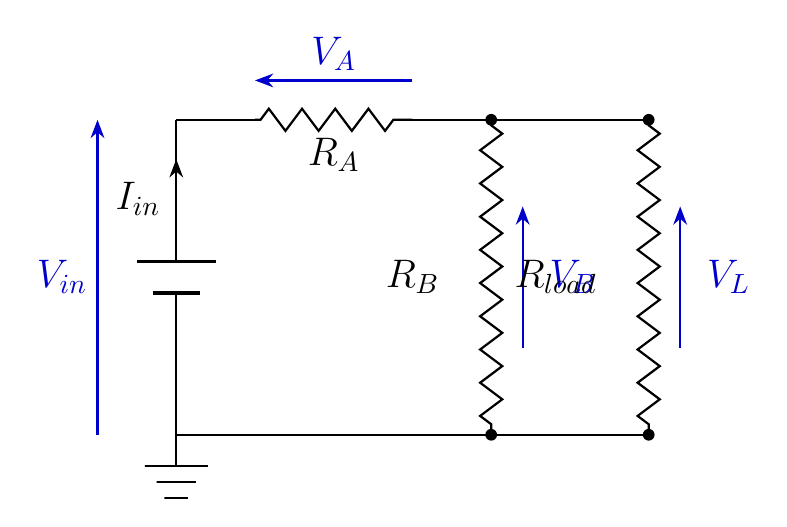
\begin{tikzpicture}[
    thick,
    font=\Large,
    myblue/.style={color=blue!80!black},
    arrow/.style={-Stealth, myblue, thick},
    resistor/.style={
        decoration={
            zigzag,
            segment length=12pt,
            amplitude=4pt,
            post=lineto,
            post length=2pt,
            pre=lineto,
            pre length=2pt
        },
        decorate,
        draw
    },
    node dot/.style={
        circle,
        fill,
        inner sep=1.5pt
    }
]

% Coordinates
\coordinate (GND_CONNECT) at (1,0);
\coordinate (V_SOURCE_TOP) at (1,4);
\coordinate (RA_START) at (2,4);
\coordinate (RA_END) at (4,4);
\coordinate (NODE_TOP_LEFT) at (5,4);
\coordinate (NODE_TOP_RIGHT) at (7,4);
\coordinate (NODE_BOTTOM_LEFT) at (5,0);
\coordinate (NODE_BOTTOM_RIGHT) at (7,0);

% Bottom (ground) wire
\draw (GND_CONNECT) -- (NODE_BOTTOM_RIGHT);

% Ground symbol
\draw (GND_CONNECT) -- ++(0,-0.4);
\draw (GND_CONNECT) ++(0,-0.4) -- ++(-0.4,0) -- ++(0.8,0);
\draw (GND_CONNECT) ++(0,-0.6) -- ++(-0.25,0) -- ++(0.5,0);
\draw (GND_CONNECT) ++(0,-0.8) -- ++(-0.15,0) -- ++(0.3,0);

% Voltage source
\draw (GND_CONNECT) -- (1,1.8);
\draw[line width=1.5pt] (1-0.3, 1.8) -- (1+0.3, 1.8);
\draw (1-0.5, 2.2) -- (1+0.5, 2.2);
\draw (1,2.2) -- (V_SOURCE_TOP);

% Top wire and Resistor RA
\draw (V_SOURCE_TOP) -- (RA_START);
\draw[resistor] (RA_START) -- (RA_END) node[midway, below=3pt] {$R_A$};
\draw (RA_END) -- (NODE_TOP_LEFT);

% Parallel branches
\draw (NODE_TOP_LEFT) -- (NODE_TOP_RIGHT);
\draw[resistor] (NODE_TOP_LEFT) -- (NODE_BOTTOM_LEFT);
\draw[resistor] (NODE_TOP_RIGHT) -- (NODE_BOTTOM_RIGHT);

% Nodes
\node[node dot] at (NODE_TOP_LEFT) {};
\node[node dot] at (NODE_TOP_RIGHT) {};
\node[node dot] at (NODE_BOTTOM_LEFT) {};
\node[node dot] at (NODE_BOTTOM_RIGHT) {};

% Labels and Arrows
% Vin and Iin
\draw[arrow] (0,0) -- (0,4) node[midway, left] {$V_{in}$};
\draw[-Stealth, thick] (1,2.5) -- (1,3.5) node[midway, left=2pt] {$I_{in}$};

% VA
\draw[arrow] (4,4.5) -- (2,4.5) node[midway, above] {$V_A$};

% VB and RB
\draw[arrow] (5.4,1.1) -- (5.4,2.9);
\node[myblue, right=6pt] at (5.4, 2) {$V_B$};
\node at (5, 2) [left=15pt] {$R_B$};

% VL and Rload
\draw[arrow] (7.4,1.1) -- (7.4,2.9);
\node[myblue, right=6pt] at (7.4, 2) {$V_L$};
\node at (7, 2) [left=15pt] {$R_{load}$};

\end{tikzpicture}
\end{document}
